\documentclass[aspectratio=169]{beamer}
\usetheme{Bruno}
\usepackage{amsmath}
\usepackage{amssymb}
\usepackage{siunitx}
\usepackage{float}
\usepackage{tikz}
\def\checkmark{\tikz\fill[scale=0.4](0,.35) -- (.25,0) -- (1,.7) -- (.25,.15) -- cycle;} 
\usepackage{url}
\usepackage[siunitx,american,RPvoltages]{circuitikz}
\ctikzset{capacitors/scale=0.7}
\ctikzset{diodes/scale=0.7}
\usepackage{tabularx}
\newcolumntype{C}{>{\centering\arraybackslash}X}
\renewcommand\tabularxcolumn[1]{m{#1}}% for vertical centering text in X column
\usepackage{tabu}
\usepackage[spanish,es-tabla,activeacute]{babel}
\usepackage{babelbib}
\usepackage{booktabs}
\usepackage{pgfplots}
\usepackage{hyperref}
\hypersetup{colorlinks = true,
            linkcolor = black,
            urlcolor  = blue,
            citecolor = blue,
            anchorcolor = blue}
\usepgfplotslibrary{units, fillbetween} 
\pgfplotsset{compat=1.16}
\usepackage{bm}
\usetikzlibrary{arrows, arrows.meta, shapes, 3d, perspective, positioning,mindmap,trees,backgrounds}
\renewcommand{\sin}{\sen} %change from sin to sen
\usepackage{bohr}
\setbohr{distribution-method = quantum,insert-missing = true}
\usepackage{elements}
\usepackage{verbatim}
\usepackage[edges]{forest}
\usepackage{etoolbox}
\usepackage{schemata}
\usepackage{appendix}
\usepackage{listings}

\definecolor{color_mate}{RGB}{255,255,128}
\definecolor{color_plas}{RGB}{255,128,255}
\definecolor{color_text}{RGB}{128,255,255}
\definecolor{color_petr}{RGB}{255,192,192}
\definecolor{color_made}{RGB}{192,255,192}
\definecolor{color_meta}{RGB}{192,192,255}
\newcommand\diagram[2]{\schema{\schemabox{#1}}{\schemabox{#2}}}

\definecolor{codegreen}{rgb}{0,0.6,0}
\definecolor{codegray}{rgb}{0.5,0.5,0.5}
\definecolor{codepurple}{rgb}{0.58,0,0.82}
\definecolor{backcolour}{rgb}{0.95,0.95,0.92}

\lstdefinestyle{mystyle}{
    backgroundcolor=\color{backcolour},   
    commentstyle=\color{codegreen},
    keywordstyle=\color{magenta},
    numberstyle=\tiny\color{codegray},
    stringstyle=\color{codepurple},
    basicstyle=\ttfamily\footnotesize,
    breakatwhitespace=false,         
    breaklines=true,                 
    captionpos=b,                    
    keepspaces=true,                 
    numbers=left,                    
    numbersep=5pt,                  
    showspaces=false,                
    showstringspaces=false,
    showtabs=false,                  
    tabsize=2
}

\lstset{style=mystyle}
\title{Instrumentación I: \\ \emph{Medidas de fuerza}\\ \emph{y vibración}}
\author{
    Juan J. Rojas, Hugo Sanchez Ortiz
}
\institute{Instituto Tecnológico de Costa Rica}
\date{\today}
\background{fig/background.jpg}
\begin{document}
\sisetup{unit-math-rm=\mathrm,math-rm=\mathrm} % change sinitx font
\sisetup{output-decimal-marker = {,}}
\maketitle

\newcommand{\blackandwhite}{white} %change this at the end

\begin{frame}{Definiciones}
    \begin{itemize}
        \item La fuerza y la aceleración están relacionadas según la 2$^\mathrm{da}$ ley de Newton
        \begin{equation*}
            \mathbf{F} = m\mathbf{a}
        \end{equation*}
        donde $\mathbf{F}$ es el vector fuerza en \si{\newton}, $\mathbf{a}$ es el vector aceleración en $\si{\meter/\second\squared}$ y  $m$ es la masa en \si{\kilo\gram}
        \item Por esta razón las formas de medir fuerza y aceleración están intrínsecamente relacionadas
    \end{itemize}
\end{frame}

\begin{frame}{¿Como medir fuerza?}
    \begin{columns}[c, onlytextwidth]
        \begin{column}{0.55\textwidth}
            \begin{itemize}
                \item Balanceando la fuerza a medir con la fuerza de una masa estándar
                \item Midiendo la aceleración que la fuerza a medir imprime sobre un masa conocida
                \item Balanceando la fuerza a medir con una fuerza generada por medios electromagnéticos
                \item Convirtiendo la fuerza en presión de fluido y midiendo esta presión
                \item Midiendo la deformación producida por la fuerza a medir en un elemento elástico
            \end{itemize}
        \end{column}
        \begin{column}{0.45\textwidth}
            \centering
            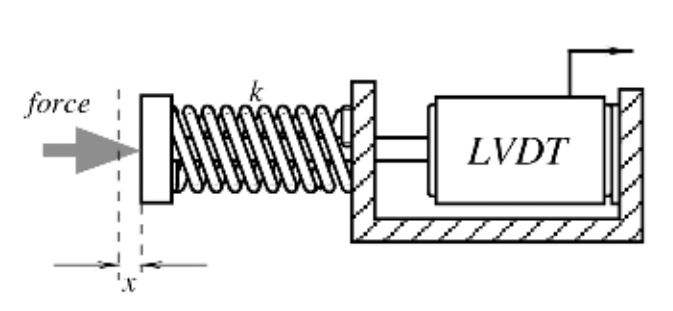
\includegraphics[width = 0.8\linewidth]{fig/Fuerza_Vibracion/fuerza1.JPG}
            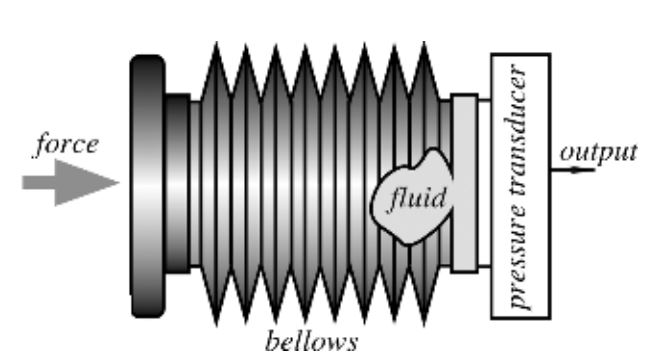
\includegraphics[width = 0.8\linewidth]{fig/Fuerza_Vibracion/fuerza2.JPG}
            \vspace{0.5cm}
            
            \tiny{Tomado de \cite{Fraden_2016}}
            
            \tiny{LVDT: linear variable differential transformer}
        \end{column}
    \end{columns}
\end{frame}


\begin{frame}{Tipos de sensores de fuerza}
    \begin{columns}[c, onlytextwidth]
        \begin{column}{0.55\textwidth}
            \begin{itemize}
                \item En la mayoría de los casos el sensor no es directo sino complejo
                \item Por ejemplo se puede hacer transducción de fuerza a distancia y luego medir la distancia con un sensor directo, como en el ejemplo de arriba. 
                \item Se puede hacer transducción de fuerza a presión y medir la presión con un sensor directo, como en el ejemplo de abajo. 
            \end{itemize}
        \end{column}
        \begin{column}{0.45\textwidth}
            \centering
            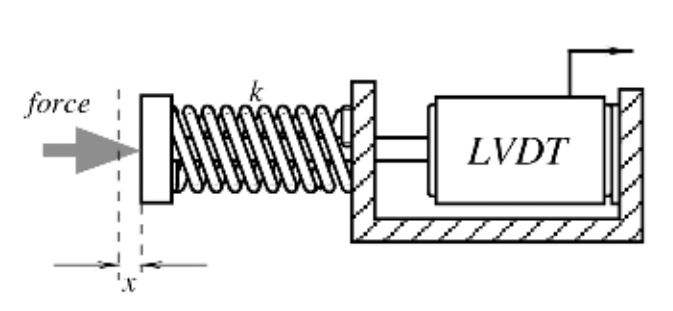
\includegraphics[width = 0.8\linewidth]{fig/Fuerza_Vibracion/fuerza1.JPG}
            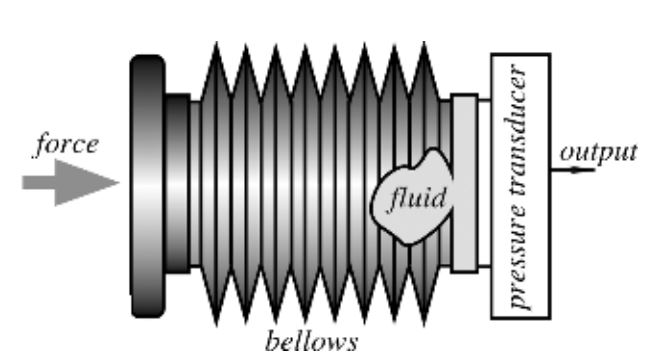
\includegraphics[width = 0.8\linewidth]{fig/Fuerza_Vibracion/fuerza2.JPG}
            \vspace{0.5cm}
            
            \tiny{Tomado de \cite{Fraden_2016}}
            
            \tiny{LVDT: linear variable differential transformer}
        \end{column}
    \end{columns}
\end{frame}

\begin{frame}{Galgas extensométricas}
    \begin{columns}[c, onlytextwidth]
        \begin{column}{0.6\textwidth}
            \begin{itemize}
                \item Una galga extensométrica es un sensor elástico resistivo cuya resistencia es una función de la deformación aplicada
                \item La relación entre la resistencia y la fuerza aplicada está definida por el effecto \emph{piezorresistivo}:
                \begin{equation*}
                    \dfrac{dR}{R} = S_e e
                \end{equation*}
                donde $S_e$ es la sensibilidad de la galga extensométrica, $e$ es la deformación unitaria -ambas cantidades adimensionales- y $R$ es la resistencia
            \end{itemize}
        \end{column}
        \begin{column}{0.40\textwidth}
            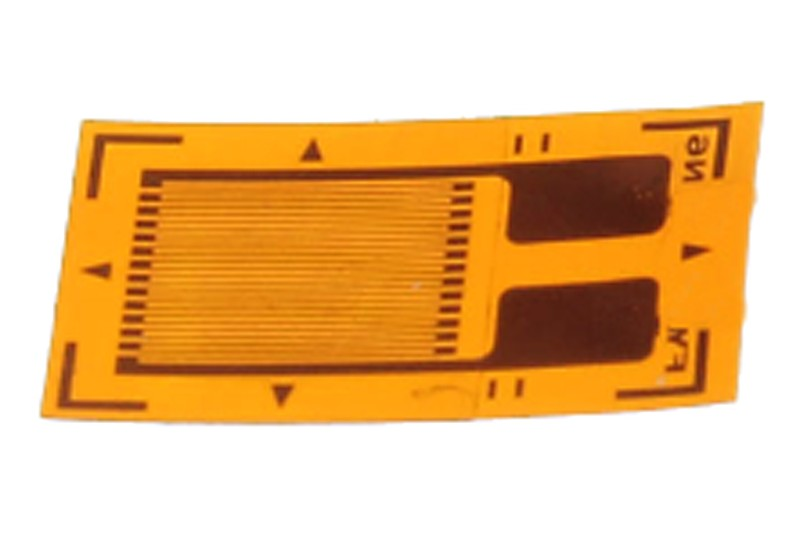
\includegraphics[width = 1\linewidth]{fig/Fuerza_Vibracion/straingauge.jpg}

            \tiny{Tomado de \href{https://www.partco.fi/16584-thickbox_default/venymaliuskaanturi350ohm.jpg}{acá}}
        \end{column}
    \end{columns}
\end{frame}

\begin{frame}{Sensores magnetoelásticos}
    \begin{columns}[c, onlytextwidth]
        \begin{column}{0.6\textwidth}
            \begin{itemize}
                \item La inducción magnética $\mathbf{B}$ y el campo magnético $\mathbf{H}$ están relacionados por:
                \begin{equation*}
                    \mathbf{B} = \mu \mathbf{H}
                \end{equation*}
                donde $\mu$ es la permeabilidad magnética del material en \si{\henry/\meter}
                \item En un sensor magnetoelástico se mide la diferencia en la permeabilidad magnetica del material al ser sometido a una fuerza externa

            \end{itemize}
        \end{column}
        \begin{column}{0.40\textwidth}
            \centering
            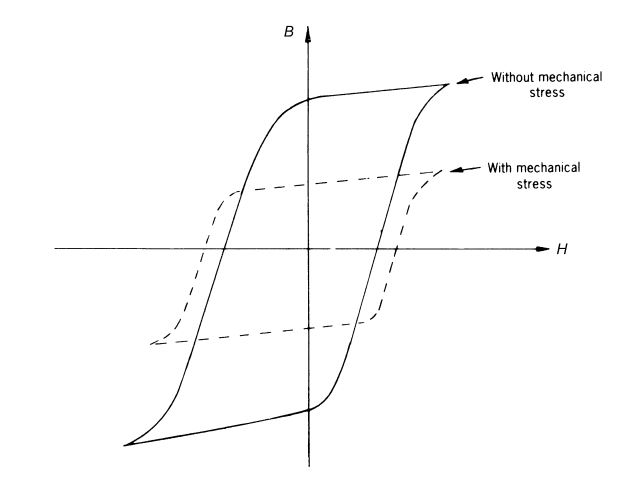
\includegraphics[width = 0.5\linewidth]{fig/Fuerza_Vibracion/magnetoelastico.JPG}
            
            \tiny{Tomado de \cite{pallas2012sensors}}
            
            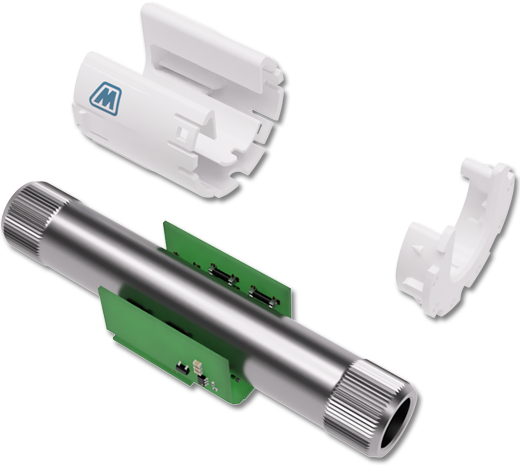
\includegraphics[width = 0.6\linewidth]{fig/Fuerza_Vibracion/Torque-Sensor.png}
            
            \tiny{Tomado de \href{https://www.methodesensor.com/industries/industrial/torque-sensing/}{acá}}
        \end{column}
    \end{columns}
\end{frame}

% \begin{frame}{Sensores de fuerza piezoeléctricos}
%     \begin{columns}[c, onlytextwidth]
%         \begin{column}{0.6\textwidth}
%             \begin{itemize}
%                 \item Una galga extensométrica es un sensor elástico resistivo cuya resistencia es una función de la deformación aplicada
%                 \item La relación entre la resistencia y la fuerza aplicada está definida por el effecto \emph{piezorresistivo}:
%                 \begin{equation*}
%                     \dfrac{dR}{R} = S_e e
%                 \end{equation*}
%                 donde $S_e$ es la sensibilidad de la galga extensométrica, $e$ es la deformación unitaria -ambas cantidades adimensionales- y $R$ es la resistencia
%             \end{itemize}
%         \end{column}
%         \begin{column}{0.40\textwidth}
%             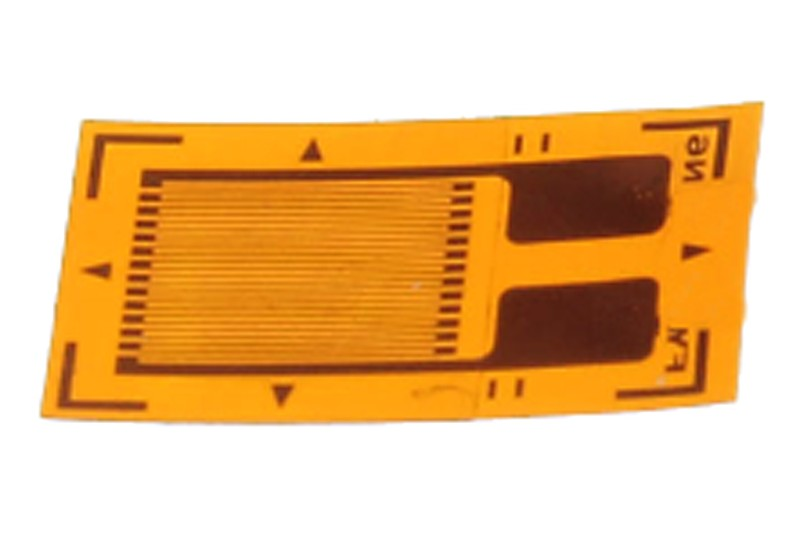
\includegraphics[width = 1\linewidth]{fig/Fuerza_Vibracion/straingauge.jpg}

%             \tiny{Tomado de \href{https://www.partco.fi/16584-thickbox_default/venymaliuskaanturi350ohm.jpg}{acá}}
%         \end{column}
%     \end{columns}
% \end{frame}

\begin{frame}{Acelerómetros}
    \begin{itemize}
        \item La vibración es un fenómeno mecánico dinámico en el que existe un movimiento oscilatorio periódico en torno a una posición de referencia 
        \item En algunos casos se puede medir aceleración no vibratoria como la que se obtiene en un impacto o un movimiento lineal
    \end{itemize}
    \begin{columns}[onlytextwidth]
        \begin{column}{0.55\textwidth}
            \begin{itemize}
                \item Los sensores que se utilizan para medir aceleración consisten en un sistema masa resorte amortiguado
                \item El acelerómetro debe ser usado en la parte plana de su curva de respuesta, lejos de su frecuencia natural
            \end{itemize}
        \end{column}
        \begin{column}{0.45\textwidth}
            \centering
            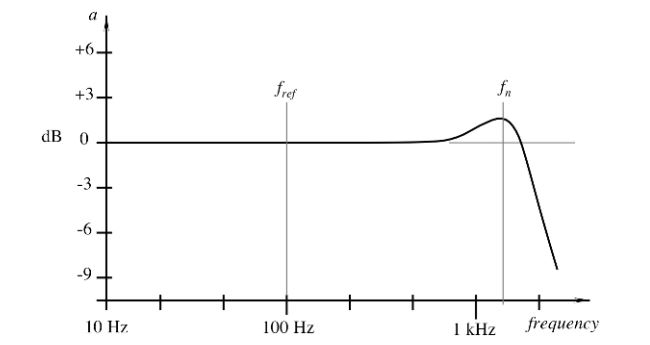
\includegraphics[width = 1\linewidth]{fig/Fuerza_Vibracion/acel.JPG}

            \tiny{Tomado de \cite{Fraden_2016}}
        \end{column}
    \end{columns}
\end{frame}

\begin{frame}{Acelerómetros capacitivos}
    \begin{columns}[c, onlytextwidth]
        \begin{column}{0.65\textwidth}
            \begin{itemize}
                \item Estos sensores consisten de una placa estática y otra placa que esta conectada a una masa inercial, estas dos placas forman un capacitor
                \item La membrana es a su vez la masa inercial, cuando se mueve modifica la capacitancia y esto se relaciona con la aceleración
                \item Típicamente se integran dos capacitores en un solo sensor para incrementar la precisión
                \item A la derecha se muestra su fabricación como sensor MEMS en silicio, con dos capacitores, uno entre la masa el \emph{cap} y otro entre la masa y la \emph{base}
            \end{itemize}
        \end{column}
        \begin{column}{0.35\textwidth}
            \centering
            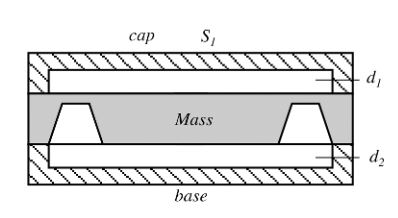
\includegraphics[width = 0.8\linewidth]{fig/Fuerza_Vibracion/memscapacc.JPG}
            
            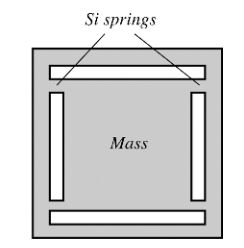
\includegraphics[width = 0.8\linewidth]{fig/Fuerza_Vibracion/memscapacc2.JPG}

            \tiny{Tomado de \cite{Fraden_2016}}
        \end{column}
    \end{columns}
\end{frame}

\begin{frame}{Acelerómetros piezoresistivos}
    \begin{columns}[c, onlytextwidth]
        \begin{column}{0.65\textwidth}
            \begin{itemize}
                \item Estos sensores consisten en galgas extensométricas que miden la deformación en los resortes del sistema masa-resorte
                \item Su precisión es mucho mayor cuando son microfabricados (MEMS)
                \item A la derecha se muestra su fabricación como sensor convencional, cuando la aceleración se aplica sobre el eje sensible la masa inercial gira en torno a la bizagra, al mismo tiempo las galgas experimentan deformación que se relaciona con la aceleración experimentada por la masa inercial
            \end{itemize}
        \end{column}
        \begin{column}{0.35\textwidth}
            \centering
            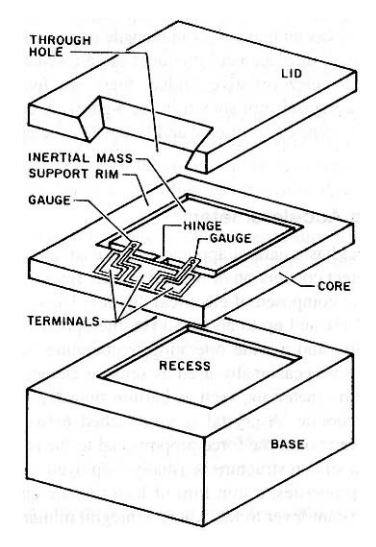
\includegraphics[width = 0.8\linewidth]{fig/Fuerza_Vibracion/memspiezoacc.JPG}
            
            \tiny{Tomado de \cite{Fraden_2016}}
        \end{column}
    \end{columns}
\end{frame}

\begin{frame}{Acelerómetros piezoeléctricos}
    \begin{columns}[c, onlytextwidth]
        \begin{column}{0.6\textwidth}
            \begin{itemize}
                \item Estos sensores consisten de un cristal piezoeléctrico intercalado entre la base y la masa inercial, la fuerza producida por la masa en el piezoeléctrico produce una señal eléctrica entre los electrodos
                \item Es un sensor directo, la energía mecanica se convierte directamente energía eléctrica
                \item Los materiales mas comunes son los materiales ceramicos piezoelectricos como el titanato de bario, el circonato-titanato de plomo (PZT) y la metaniobita de plomo
            \end{itemize}
        \end{column}
        \begin{column}{0.4\textwidth}
            \centering
            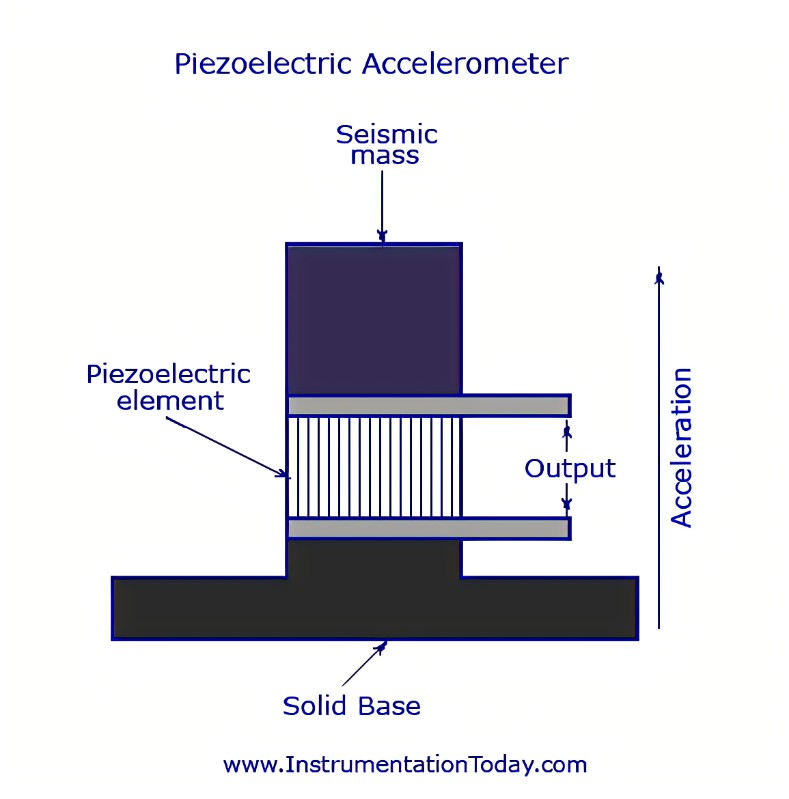
\includegraphics[width = 1\linewidth]{fig/Fuerza_Vibracion/piezo.jpg}
            
            \tiny{Tomado de \href{www.instrumentationtoday.com}{acá}}
        \end{column}
    \end{columns}
\end{frame}

\begin{frame}{Acelerómetros de gas caliente}
            \begin{itemize}
                \item Estos sensores usan un gas caliente como masa inercial
                \item El gas se calienta en el centro del sensor y se mide la temperatura en dos extremos equidistantes, los cambios de temperatura entre los extremos representan aceleración de la masa de gas, pues sin aceleración la distribución de la temperatura debe ser uniforme
                \item Estos sensores son microfabricados (MEMS)
            \end{itemize}
            \centering
            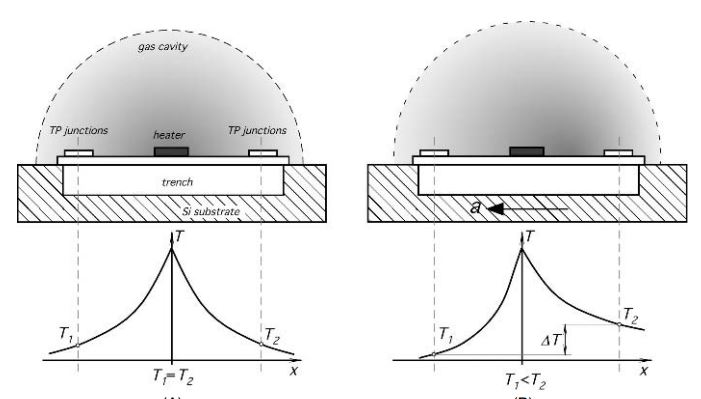
\includegraphics[width = 0.5\linewidth]{fig/Fuerza_Vibracion/memsheatedgasacc.JPG}
            \tiny{Tomado de \cite{Fraden_2016}}
\end{frame}

\begin{frame}{Referencias}
\bibliographystyle{ieeetr}
\footnotesize
\bibliography{comunes/referencias}
\end{frame}

\end{document}